%clase del documento
\documentclass[a4paper,12pt]{book}

%paquete de idioma y codificación de caracteres
\usepackage[spanish]{babel}
\usepackage[utf8]{inputenc}
\usepackage{afterpage}

%figuras en un lugar determinado
\usepackage{float}

\usepackage{cite} % para contraer referencias
\usepackage{fancyhdr} % para encabezados y pie de pagina

% soporte gráfico
\usepackage{graphicx} % figuras
\usepackage{subfigure} % subfiguras
\graphicspath{ {images/} }

%indice dentro de secciones
\usepackage{minitoc}

%datos del documento
\author{Ignacio Agüero Salcines}
\title{Especificación Gráfica de Procesos de Recuperación de Datos en LUCA}

\setcounter{tocdepth}{5}
\setcounter{secnumdepth}{5}



\begin{document}
	
	
	\pagestyle{empty}
	\dominitoc% Inicializacion
	\tableofcontents
	\cleardoublepage
	
	\pagestyle{plain}
	
	\listoffigures
	\listoftables
	\thispagestyle{empty}
	\cleardoublepage
	
	\pagenumbering{roman}
	\chapter*{Agradecimientos}
	Me gustaría dar agradecimientos a mi familia y facultad, ya que sin ellos esto no habría sido posible nada de estos.
	
	\vspace{5mm}
	
	\noindent Es importante agradecer también a CIC Consulting Informático por permitirme la oportunidad de realizar el desarrollo del proyecto en su empresa, sin olvidarme de mis compañeros de LUCA, que han sido un gran apoyo durante el mismo..
	
	\vspace{5mm}
	
	\noindent Para finalizar, me gustaría gradecer a mi mentor Pablo, por guiarme durante el desarrollo del proyecto con eficacia y ayudarme a afrontar este trabajo de fin de grado.
	\cleardoublepage
	
	\clearpage
	
	\chapter*{Resumen}
	Las empresas actuales utilizan ya no un único sistema de información que de	soporte a sus procesos de trabajo, sino un  ecosistema de sistemas información que dan soporte a diferentes procesos de negocio ejecutados dentro de dicha organización. Como consecuencia de esta nueva situación, cuando un usuario	quiere obtener una información concreta cuyos datos residen en varios de estos
	sistemas, necesita acceder a cada uno de estos sistemas, extraer de cada sistema la información que precisa, filtrarla y unificarla para finalmente	obtener los datos requeridos.
	
	\vspace{5mm}
	
	Por ejemplo, una tienda de electrodomésticos podría tener sistemas informáticos diferentes para el departamento de atención al cliente, para el departamento técnico de postventa y para el departamento de compras y adquisiciones.Por tanto, para conocer el estado actual de una reparación, podríamos necesitar:
		\begin{itemize}
			\item  Acceder al primer sistema para obtener el identificador de la incidencia y en qué fase de su gestión se encuentra.
			\item  Comprobado que la incidencia está actualmente en reparación, recuperaríamos otro sistema el estado detallado de la reparación, comprobando que está a la espera de una pieza.
			\item Finalmente accederíamos al sistema de compra y adquisiciones para comprobar cuando está prevista la entrega de dicha pieza. Los sistemas de almacenamiento de la información puede ser diversos, incluyendo desde un servicio web, una base de datos relacional, un repositorio de ficheros accesible vía FTP o una base de datos NoSQL.
		\end{itemize}
	
	\vspace{5mm}
	
	El objetivo de este proyecto es facilitar dicho proceso de composición al usuario mediante el desarrollo de un mecanismo gráfico para la especificación de estos procesos de composición de consultas.
	

	\vspace{5mm}
	
	\textbf{Palabras clave}: 
	\cleardoublepage
	
	\clearpage
	
	\chapter*{Preface}

	

	\textbf{Keywords}:
	\cleardoublepage
	
	\pagenumbering{arabic}
	\setcounter{page}{1}
	
	\clearpage
	
	\chapter{Introducción}
	
	Este capítulo del documento se propone a describir, en leves pinceladas, los objetivos principales que el proyecto debe de completar.
	
		\section{Introducción}
	
	
			En los últimos años, el volumen de datos que una empresa o entidad necesita y/o es capaz de gestionar o manipular, ha aumentado de forma vertiginosa. Además del volumen de datos a manipular, nos damos cuenta de que para acceder a lo diversos datos es necesario muchas veces establecer comunicaciones con los diversos recursos existentes para alcanzar el objetivo.
			
			\vspace{5mm}
			
			
			 Con el objeto de facilitar este proceso de recuperación de información almecenada en sistemas y fuentes de datos hetereogéneas, dentro de la empresa	CIC, se está desarrollando una aplicación denominada LUCA. Para	facilitar este proceso de recuperación de información, LUCA proporciona un lenguaje común para todas las fuentes de datos a unificar, permitiendo al
			usuario abstraerse de los detalles de cada fuente.
			
			\vspace{5mm}
			
			 Actualmente LUCA proporciona mecanismos o abstracciones para permitir al	usuario recuperar de manera uniforme información de diferentes fuentes de datos. No obstante, LUCA actualmente sólo es capaz recuperar información de una única fuente de datos a la vez. Por tanto, cuando es necesario combinar información procedente de distintas fuentes, el propio usuario es el que debe realizar dicho	proceso de composición, ejecutando cada consulta a mano, y utilizando las salidas de cada una de ellas como las entradas de las siguientes.
			 
			 \vspace{5mm}
			 
			 El objetivo de este proyecto es facilitar dicho proceso de composición al usuario mediante el desarrollo de un mecanismo gráfico para la especificación de estos procesos de composición de consultas.
			 
	 
	 	\section{Planificación del proyecto}
	 	
	 	En este apartado se describe la metodología de desarrollo que ha sido utilizada para la cumplimentación del proyecto. 
	 	
	 	\vspace{5mm}
	 	
	 	
	 	En el proyecto se optó por utilizar una metodología en cascada, en la que de forma iterativa se va puliendo el producto hasta completar los requisitos y objetivos establecidos.
	 	
	 	\vspace{5mm}
	 	
	 	\begin{figure}[h]
	 		\centering
	 		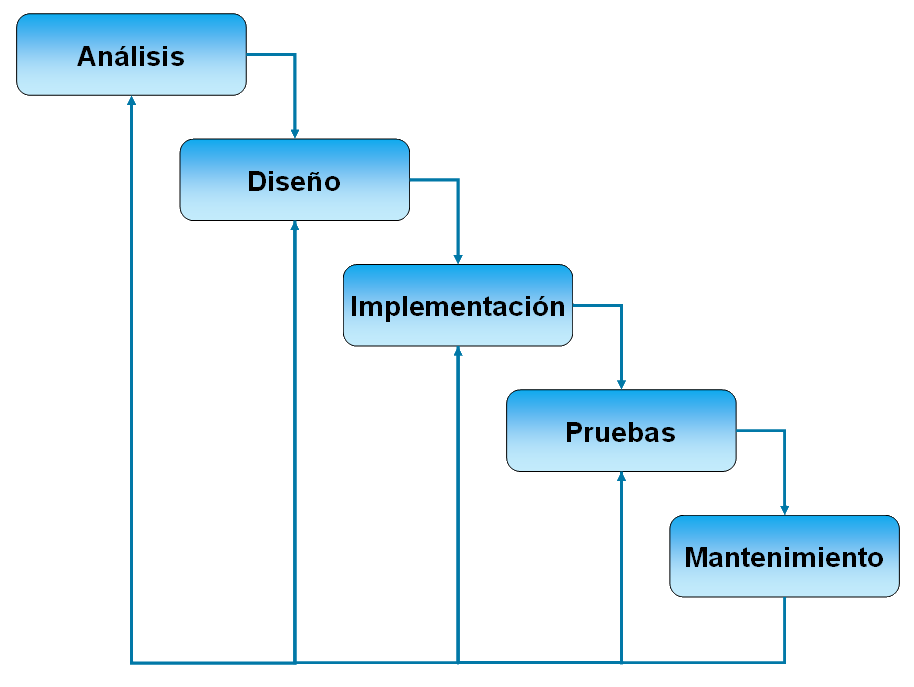
\includegraphics[scale=0.5]{modelo-en-cascada.png}
	 		\caption{Metodología En Cascada}\label{fig:modelo-en-cascada}
	 	\end{figure}
 	
 		\vspace{5mm}
 	
 		Acorde a la imagen mostrada previamente, la primera etapa de la metodología que se llevo a cabo para la cumplimentación del proyecto fue el análisis de los requisitos y objetivos del proyecto. El objetivo de esta etapa es describir de forma detallada el conjunto del requisitos y funcionalidades necesarias para la satisfacción del stakeholder y la completitud del sistema.
 		
 		\vspace{5mm}
 		
 		Una vez en posesión de la especificación de requisitos, el siguiente paso fue definir el diseño arquitectónico del proyecto en bloques independientes que puediesen ser elaborados y probados de forma aislada. Otro requisito importante que se tuvo que tener en cuenta fue, que el producto debe de estar diseñado para poder hacer frente a futuros incrementos.
 		
 		\vspace{5mm}
 		
 		Utilizando el diseño arquitectónico ya definido, se focalizó el esfuerzo en el diseño de la aplicación. En esta se tuvo en cuenta que se pretenden realizar dos elaboraciones o componentes software:
 		
 		\vspace{5mm}
 		
 		\begin{itemize}
 			\item En una primera instancia se desarrollara un componente genérico cuya funcionalidad es de índole gráfica, por lo que no precisa de una desarrollo en capas común, ya que consta unicamente de un modelo de datos y una implementación web a través del Framework GO.JS, así la integración con Vaadin\cite{vaadin}.
 			
 			\item En una segunda instancia se desarrollará una aplicación incremento del producto actual ya elaborado llamado LUCA. El cuál sigue un patrón MVP \cite{mvp}, y esta elaborado en Spring\cite{spring}.
 		\end{itemize}
 	
 		\vspace{5mm}
 		
 		Para aplicación desarrollado con Spring, se creó una base de datos relacional asociada, la cuál servirá de fuente de persistencia de los datos almacenados.
 		
 		\vspace{5mm}
 		
 		Tras la especificación de la base de datos comenzó un proceso iterativo de implementación, verificación y pruebas en el que en función de los diversos requisitos se fue completando el proyecto.
 		 
	 
	 
		\section{Estructura del documento}
		
		Esta sección se propone describir la ingeniería de requisitos llevada a cabo, así como, profundizar en el diseño arquitectónico. También como introducción inicial, se relatará de forma breve y concisa la librería javascript GO.JS y el framework Vaadin.
		
		\vspace{5mm}
		
		 En primera instancia explicará el proceso de captura y especificación de requisitos llevado a cabo, así como, la toma de decisiones seguidas. También se centrará en detallar y explicar las decisiones para la especificación de la base de datos, que deberán de estar de acuerdo con las implementación actuales de las bases de datos de LUCA, y con la especificacion basada en Spring.	Por último se explicará el proceso de desarrollo de las capas de repositorio, servicios y presentación.
		
		
		
	 
	  \clearpage
	 
	

	\chapter{Ingeniería de Requisitos}
	
	Este capítulo describe el proceso de captura de requisitos, así como, el modelado de los requisitos tanto funcionales como no funcionales.
	
	\minitoc
	
	
	
		\section{Introducción}
		
		El capítulo actual se propone explicar de forma detallada la fase de ingeniería de requisitos, en la que se recoge toda la información necesaria relativa a los requisitos para poder presentar al stakeholder los objetivos o requerimentos que debe de tener la aplicación para poder considerarse como completada.
		
		\vspace{5mm}
		
		Por tanto, teniendo en cuenta lo citado anteriormente, este capítulo tratará primero el proceso de captura de requisitos llevado a cabo, para posteriormente, mostrar y detallar el modelado de requisitos subyacente de la etapa anterior.
		
		\section{Captura de requisitos}
		
		En la presente sección se describe el proceso de identificación de requisitos que nuestra aplicación debe de completar o satisfacer. 
		
		\vspace{5mm}
		
		Dado que la aplicación a construir es un incremento de un producto ya existente, no hace falta identificar la fuente de los requisitos ya que es el propio gerente o impulsor de dicho incremento el stakeholder, junto con el jefe del proyecto, los objetivos conjuntos de la captura de información y de los propios requisitos.
		
		\vspace{5mm}
		
		A raíz de una demostración del producto actual LUCA, y de la reunión para la captura de requisitos con el gerente y de la empresa CIC, así como del jefe de proyecto bajo el que estuvo supervisado el proyecto actual, se muestra el resultado del proceso de la captura de requisitos llevada a cabo. 
		
		\vspace{5mm}
		
		Cabe explicar también, que este proyecto se funda en la implementación o desarrollo de dos componentes. Uno  representa una herramienta focalizada en el ámbito grafico para la creación, borrado y actualización, en términos genrales, manipulación gráfica de los elementos constituyentes del proyecto. El otro represente un proyecto incremento del actual producto LUCA, centrado en la gestión de los procesos y elementos hijos.
		
		\vspace{5mm}
		A continuación se muestra, por cada componente, una tabla desglosando los diferentes requisitos , y posteriormente, una breve explicación general del mismo:
		
		
		\begin{table}[H]
			\begin{center}
				\begin{tabular}{|l|l|}
					\hline
					Referencia & Requisito \\
					\hline \hline
					REF-01 & Los usuarios podrán consultar los datos referentes a los diversos elementos o cajas. \\ \hline
					REF-02 & Los usuarios podrán modificar los datos de los elementos. \\ \hline
					REF-03 & Los usuarios podrán persistir los nuevos elementos creados. \\ \hline
					REF-04 & Los usuarios podrán concatenar los diferentes elementos ( procesos, subprocesos y condicionales) para formar una jerarquía de elementos con una semántica propia\\ \hline
					REF-05 & Los usuarios podrán persistir, a partir de las consultas almacenadas en el sistema, una jerarquía de procesos constituidos por elementos. \\ \hline

				\end{tabular}
				\caption{Conjunto de Requisitos del Proyecto}
				\label{tabla:requisitosProceso}
			\end{center}
		\end{table}
	
		\vspace{5mm}

		El usuario deberá de ser capaz de interactuar con los diferentes elementos existentes como son las consultas almacenadas. Desde poder crear conjunto de consultas anidadas mediante sus entradas y salidas para obtener una salida final objetivo, hasta poder modificar o eliminar los esquemas o procesos ya almacenados.
	
	
		\begin{table}[H]
			\begin{center}
				\begin{tabular}{|l|l|}
					\hline
					Referencia & Requisito \\
					\hline \hline
					REF-01 & Los usuarios deberán de ser capaces de enlazar los diferentes elementos entre sí. \\ \hline					
					REF-02 & Los usuarios deberán de ser capaces de seleccionar de diferentes formas los elementos así como las diversas opciones relacionadas con el \\ \hline					
					REF-03 & Los usuarios deberán de ser capaces mover e interactuar con los diferentes elementos.\\ \hline
				\end{tabular}
				\caption{Conjunto de Requisitos del Componente Gráfico}
				\label{tabla:requisitosHerramientaProceso}
			\end{center}
		\end{table}
	
		\vspace{5mm}
	
		El usuario podrá realizar acciones de forma gráfica como son la selección o arrastrado de los diversos elementos que conforman la estructura semántica del componente.
	
	
		
		
		
	
	
		\section{Modelado de requisitos}
	Este apartado muestra el proceso de modelado de requisitos, los cuales fueron especificados en el apartado anterior, así como la explicación y especificación del mismo.
	
	//TODO
	metodologia usada para la especificacion de los casos de usos de klaus pohl\\
	
	caso de uso: gestionar procesos, alta baja etc

	
	
	\clearpage
	

	 \chapter{Análisis y documentación}
	 Este capítulo describe el proceso de adquisición de conocimientos necesarios para poder llevar a cabo el proceso de diseño arquitectónico y de construcción o implementacíon de la aplicación. De esta fomra se puede realizar una planificación mas cercana a la realidad y partir de unos conocimientos mínimos para empezar a elaborar el proyecto.
	 
	 \minitoc
	 
	 	\section{GO.JS}
	 		
	 		
	 		\begin{figure}[H]
	 			\centering
	 			
\includegraphics[scale=1]{gojs.jpeg}
	 			\caption{GO.JS Logo}\label{fig:gojs}
	 		\end{figure}
	 	
	 	
	 		\subsection{¿Qué es GO.JS?}
	 			Go.JS \cite{gojs} es una biblioteca de JavaScript con múltiples funciones para implementar diagramas interactivos personalizados y visualizaciones complejas en navegadores y plataformas web modernos.
	 	
	 		\subsection{¿Porqué GO.JS?}
	 		 GoJS facilita la construcción de diagramas de JavaScript de nodos, enlaces y grupos complejos con plantillas y diseños personalizables.
	 		
	 		
	 		\subsection{Características}
	 		GoJS ofrece muchas características avanzadas para la interactividad del usuario, tales como arrastrar y soltar, copiar y pegar, edición de texto en el lugar, información sobre herramientas, menús contextuales, diseños automáticos, plantillas, vinculación y modelos de datos, administración de estado transaccional y deshacer, paletas , vistas generales, controladores de eventos, comandos y un sistema de herramientas extensible para operaciones personalizadas.
	 		
	 	
	 		\subsection{Explicación}
	 		GoJS ofrece muchas características avanzadas para la interactividad del usuario, tales como arrastrar y soltar, copiar y pegar, edición de texto en el lugar, información sobre herramientas, menús contextuales, diseños automáticos, plantillas, vinculación y modelos de datos, administración de estado transaccional y deshacer, paletas , vistas generales, controladores de eventos, comandos y un sistema de herramientas extensible para operaciones personalizadas.
	 
	 
	 	\section{Vaadin}
	 	
	 		\begin{figure}[H]
	 			\centering
	 			
\includegraphics[scale=1]{Vaadin-logo.png}
	 			\caption{Vaadin Logo}\label{fig:Vaadin-logo}
	 		\end{figure}
 		
 			\subsection{¿Qué es GO.JS?}
 				Vaadin\cite{vaadin} es un framework de desarrollo de SPA que permite escribir el código de dichas aplicaciones en Java o en cualquier otro lenguaje soportado por la JVM 1.6+. Esto permite la programación de la interfaz gráfica en lenguajes como Java 8, Scala o Groovy, por ejemplo.
 			
 			\subsection{Características}
 				Uno de las características diferenciadores de Vaadin es que, contrario a las librerías y frameworks de JavaScript típicas, presenta una arquitectura centrada en el servidor, lo que implica que la mayoría de la lógica es ejecutada en los servidores remotos. Del lado del cliente, Vaadin está construido encima de Google Web Toolkit, con el que puede extenderse.
 	
 			\subsection{Aplicación}
 				En este proyecto, Vaadin se encargara de realizar la comunicación entre el cliente y el servidor. De esta forma, será capaz de enviar y recibir datos, eventos y peticiones entre el componente Javascript (cliente) y el servidor.
 			
 			
	 			\begin{figure}[H]
	 				\centering
	 				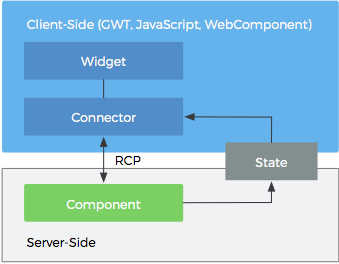
\includegraphics[scale=1.5]{schema.png}
	 				\caption{Esquema Cliente-Servidor}\label{fig:schema}
	 			\end{figure}
 			
	
	
	\section{Spring}
	
		\begin{figure}[H]
			\centering
			
\includegraphics[scale=0.5]{spring.png}
			\caption{Spring Logo}\label{fig:spring}
		\end{figure}
		
		Spring\cite{spring} es un Framework que proporciona un modelo de programación y configuración integral para aplicaciones empresariales modernas basadas en Java y en cualquier tipo de plataforma de implementación. Un elemento clave de Spring es el soporte de infraestructura a nivel de aplicación, ya que Spring se centra abstraer a las aplicaciones empresariales del uso de diferentes frameworks para que los equipos puedan centrarse en la lógica empresarial a nivel de aplicación, sin lazos innecesarios con entornos de implementación específicos.
	
	
	\clearpage
	
	\chapter{Diseño Arquitectónico}
	
	Tras haber adquirido la información suficiente respecto al conjunto de requisitos objetivos de satisfacción, y del conjunto de tecnologías que deben de integrarse en el proyecto, se muestra a continuación la especificación del diseño arquitectónico.
	
	\vspace{5mm}
	
	El diseño arquitectónico va a describir tanto la estructura arquitectónica del componente de procesos implementado con GO.js, tanto su integración en el producto LUCA, el cual, requiere de un diseño paralelo que implementar.
	
	
	\minitoc
	
	
	Para poder diferenciar estos dos diseños, el componente que implementa GO.JS se nombrará como 'Process Component' y el diseño del producto LUCA que integra el Process Component se llamara 'LUCA Process'.
	
		\section{Process Component}
		
		
		\begin{figure}[H]
			\centering
			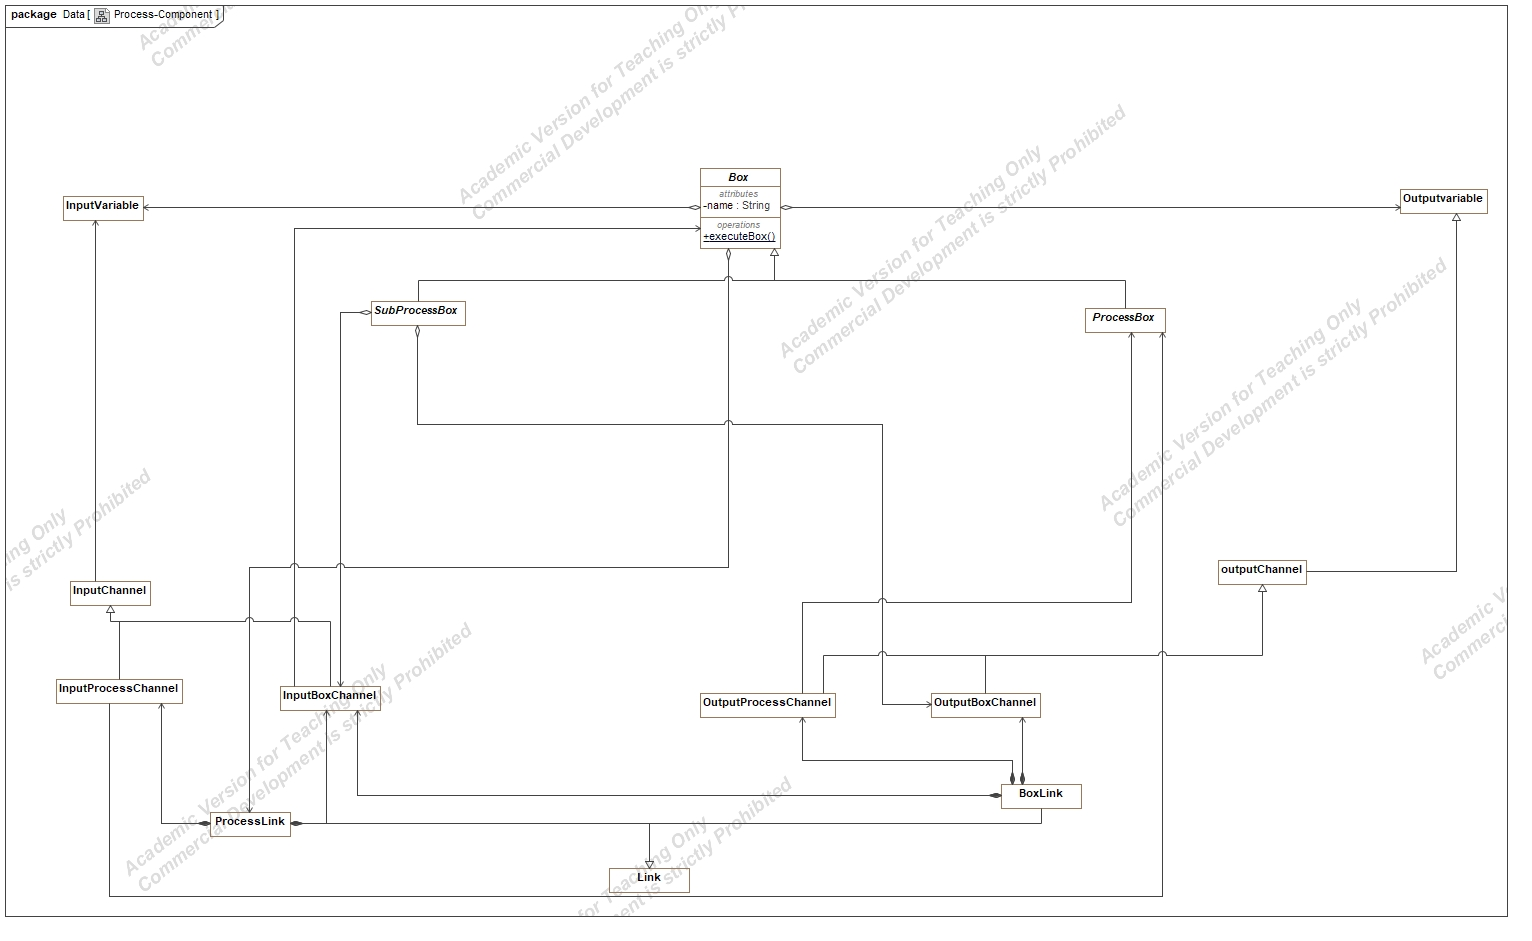
\includegraphics[scale=0.25]{Process-Component.jpg}
			\caption{Diagrama de clases}\label{fig:Process-Component}
		\end{figure}
		
		
		\section{Luca Process}
		
		\begin{figure}[H]
			\centering
			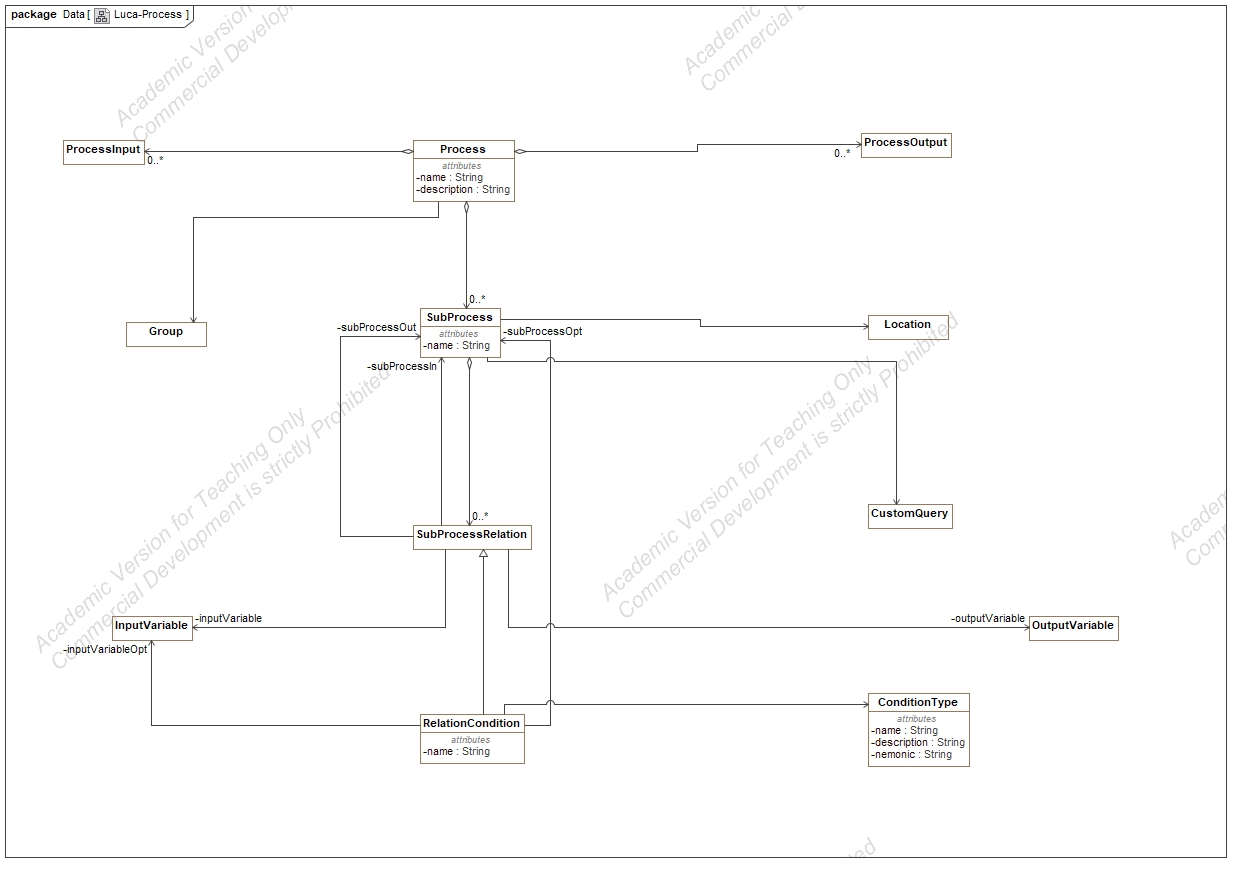
\includegraphics[scale=0.35]{Luca-Process.jpg}
			\caption{Diagrama de clases}\label{fig:Luca-Process}
		\end{figure}
	
	\clearpage
	
	\chapter{Implementación}
	
	El capítulo presente describe el proceso llevado a cabo para realizar la implementación tanto del componente gráfico (Process-Component) como del componente de Luca (Luca-Process).
	
	\vspace{5mm}
	
	A continuación, se declara un breve desglose de los dos componentes con los fragmentos que han sido implementados para poder satisfacer los el diseño arquitectónico.
	
	\begin{figure}[H]
		\centering
		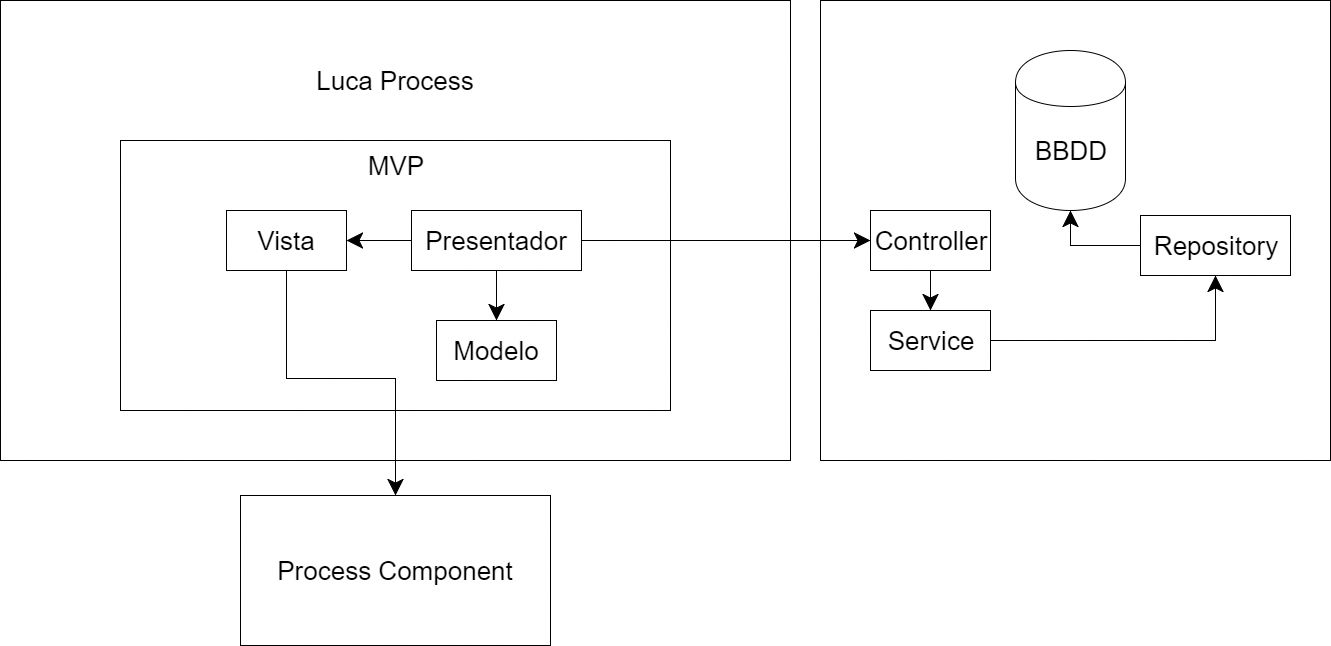
\includegraphics[scale=0.25]{esquema_proyecto.png}
		\caption{Estructuración en módulos}\label{fig:esquema_proyecto}
	\end{figure}
	
	\minitoc
	
		\section{Process-Component}
		
		Este fragmento del proyecto o componente se dedica exclusivamente al apartado gráfico, el cuál posee una sintaxis ya definida en el apartado del diseño arquitectónico.
		
		
		\vspace{5mm}
		
		
		Este componente es una herramienta que se dedica a proveer métodos para interactuar con él y además es capaz mediante escuchadores de avisar a los clientes que lo requieran sobre los eventos ocurridos sobre la interfaz gráfica.
		
		\vspace{5mm}
		
		Su implementación se centra en dos pilares centrales. Por una parte se ha realizado un proyecto Vaadin encargado de mantener el estado de la aplicación gráfica, y por otro lado un conjunto de ficheros Javascript implementados sobre GO.JS que se encargan de modificar el entorno gráfico mediante sentencias .
		\begin{itemize}
			\item Proyecto Vaadin
			\subitem Este proyecto es el encargado de crear los metodos necesarios para interactuar desde el exterior con el esquema creado previamente. Además debe de permitir insertar escuchadores para los eventos proporcionados desde GO.JS, de forma que se pueda establecer dos direcciones de comunicaciones. Una desde el exterior con el proyecto Vaadin y este con el conector y directamente con el entorno gráfico de GO.JS, y otro desde interacción con los eventos (por parte del usuario) desde el fichero Javascript de configuración (explicado en el apartado posterior), con el conector y este con el estado, es decir, con el proyecto Vaadin.
			
			\item Ficheros Javascript
			\subitem Existe un primer fichero que permite configurar el esquema gráfico que se va a llevar a cabo (Procesos, Subprocesos, InputVariables, OutputVariables ...), así como todo el resto de propiedades gráficas, ademas de ser capaz de lanzar eventos preconfigurados.
			
			\vspace{5mm}
			
			El segundo fichero esencial para el funcionamiento de esta estructura es el fichero conector. Este es el encargado de declarar y configurar todos los eventos que se pueden lanzar, además de ser el encargado de realizar todos los metodos CRUD \footnote{CRUD es el acrónimo de crear, leer, actualizar y borrar, en esete contexto significa el conjunto de métodos para poder realizar dichas acciones sobre los distintos elementos existentes.}necesarios para que puedan interactuar con las propiedades configuradas en el primer fichero citado previamente.
		\end{itemize}
	
		Esta imagen trata de  resumir el esquema de actuación que se lleva a cabo para la comunicación entre los distinto elementos del Process-Component.
		
		\begin{figure}[H]
			\centering
			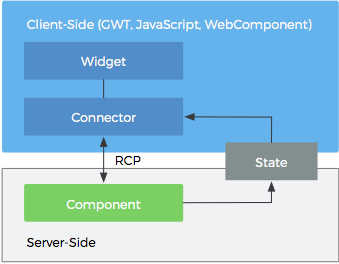
\includegraphics[scale=1.25]{schema.png}
			\caption{Estructuración en módulos}\label{fig:schema}
		\end{figure}
		
		
		\section{Luca-Process}
	
	\clearpage
	
	
	\chapter{Pruebas}
	
	Este capítulo describe el proceso llevado a cabo de diseño y de implementación de las pruebas realizadas. Para este proyecto se ha decidido llevar a cabo pruebas unicamente de ámbito funcional, basándose en el modelo de pruebas en tres fases.
	
	\vspace{5mm}
	
	Todo el conjunto de pruebas utilizan el módulo JUnit \cite{jpaunit} para verificar la correcta ejecución de las pruebas.
	
	\minitoc
	
		\section{Pruebas Unitarias}
		
		Las pruebas unitarias se focalizan en la capa de persistencia o repositorio del proyecto, debido a que en este caso, la capa de repositorio utiliza el framework JPA \cite{jpa}, el cuál garantiza ya una funcionalidad, no ha sido necesario realizar pruebas unitarias.
		
		\section{Pruebas de Integración}
		
		Las pruebas de integración se han realizado sobre la capa de negocio, concretamente la capa de servicios, del proyecto.
		
		\vspace{5mm}
		
		En estas pruebas se utilizará la capa de repositorio para persistir los elementos. Además, para cada test, se ha establecido un fichero sql que es tomado al inicio de cada test para establecer unos valores de entrada previos en la base de datos y asi poder ser utilizados dentro del test. El proceso de desarrollo de las pruebas se ha repartido en tres fases:
		
		\begin{itemize}
			\item Pruebas CRUD
			\subitem En este grupo de pruebas se ha comprobado que se puedan llevar a cabo los diversos tipos de operaciones sobre todo el conjunto de clases objetivo de persistencia. Un ejemplo de este tipo de pruebas es el siguiente: 
			
			\begin{figure}[H]
				\centering
%				\includegraphics[scale=1]{pruebasIntegracionSimples.png}
				\caption{Pruebas de Integración del la clase Process}\label{fig:pruebasIntegracionSimples}
			\end{figure}
			
			\item Guardar a partir de estructura
			\subitem Esta parte comprueba que funciona la capacidad de la aplicación de guardar toda una estructura de clases a partir de una clase padre que contiene la información necesaria para persistir toda la estructura. Se caracteriza por recibir un objeto perteneciente al Process-Component, el cual provee de toda las clases e información para poder hacer una conversión a las clases del Luca-Process.
			
			
			\begin{figure}[H]
				\centering
%				\includegraphics[scale=1]{pruebasIntegracionComplejas.png}
				\caption{Prueba de Integración de Guardado Estructural}\label{fig:pruebasIntegracionComplejas}
			\end{figure}
		
			\item Cargar un proceso
			\subitem En construcción...
			
		\end{itemize}
				
		\section{Pruebas de Sistema}
		
		\section{Pruebas de Aceptación}
	
	
	\clearpage
	
	
	
	\chapter{Conclusiones}
	
	Para finalizar, a continuación se relatan las conclusiones sacadas tras el transcurso y ejecución del proyecto.
	
	\vspace{5mm}
	
	El objetivo principal del proyecto consistía en crear un proyecto que fuese capaz de permitir al usuario de forma gráfica y sencilla crear una jerarquía de procesos para enlazar las diferentes consultas existentes en el producto LUCA. 
	
	\vspace{5mm}
	
	Tras completar con éxito la implementación del proyecto, se implanto en el producto LUCA, para comprobar el correcto funcionamiento e integración y comprobar así la correcta y eficiente satisfacción de los requerimientos impuestos al proyecto.
	
	\vspace{5mm}
	
	En el apartado persona, ha sido una gran oportunidad poder realizar este proyecto en una empresa como es CIC, ya que ayuda a tener una constancia y hábito de trabajo y nos prepara para el ámbito empresarial. Además ha sido muy satisfactorio poder trabajar con mas de una tecnología ya que aporta muchos conocimientos.


	\clearpage
	
	\bibliographystyle{acm}
	\bibliography{Bibliografia}
	

\end{document}


